\documentclass[mathserif]{beamer}
\usetheme{Berkeley}
\usecolortheme{albatross}
\usepackage{listings}
\usepackage{pgf}
\usepackage{qtree}
\usepackage{tikz}
\usetikzlibrary{shapes, arrows}
\usepackage{gb4e}

\title{Constructing a Knowledge Base on Aging}
\subtitle{An Automated Approach}
\author{Mark Farrell}
\institute
{

Bioinformatics Researcher \and

\inst{}%
Center for Research and Education on Aging \\
Lawrence Berkeley National Laboratory \\
University of California, Berkeley

}

%\logo{
\includegraphics[width=30px]{images/logo.png}}

\date{September 4th, 2014}
\subject{Bioinformatics}

\AtBeginSection[]
{
\begin{frame}
\frametitle{Outline}
\tableofcontents[currentsection]
\end{frame}
}

\lstset{
basicstyle=\small\sffamily,
columns=fullflexible,
showstringspaces=false
}

\noautomath

\begin{document}

\begin{frame}
\titlepage
\end{frame}

\section{About Me}

\begin{frame}

\frametitle{Who I am}
\framesubtitle{Mark Farrell}

\centering

\begin{tabular}{c c}
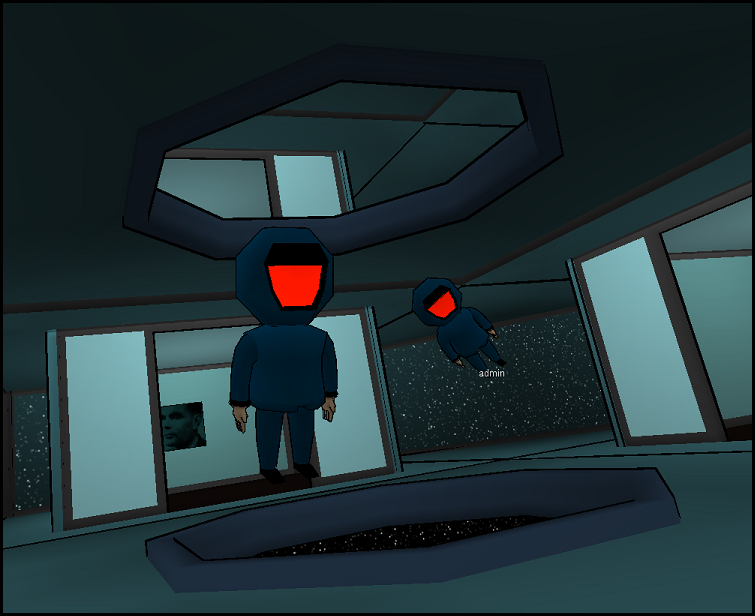
\includegraphics[width=0.30\linewidth]{images/starfall.png}&
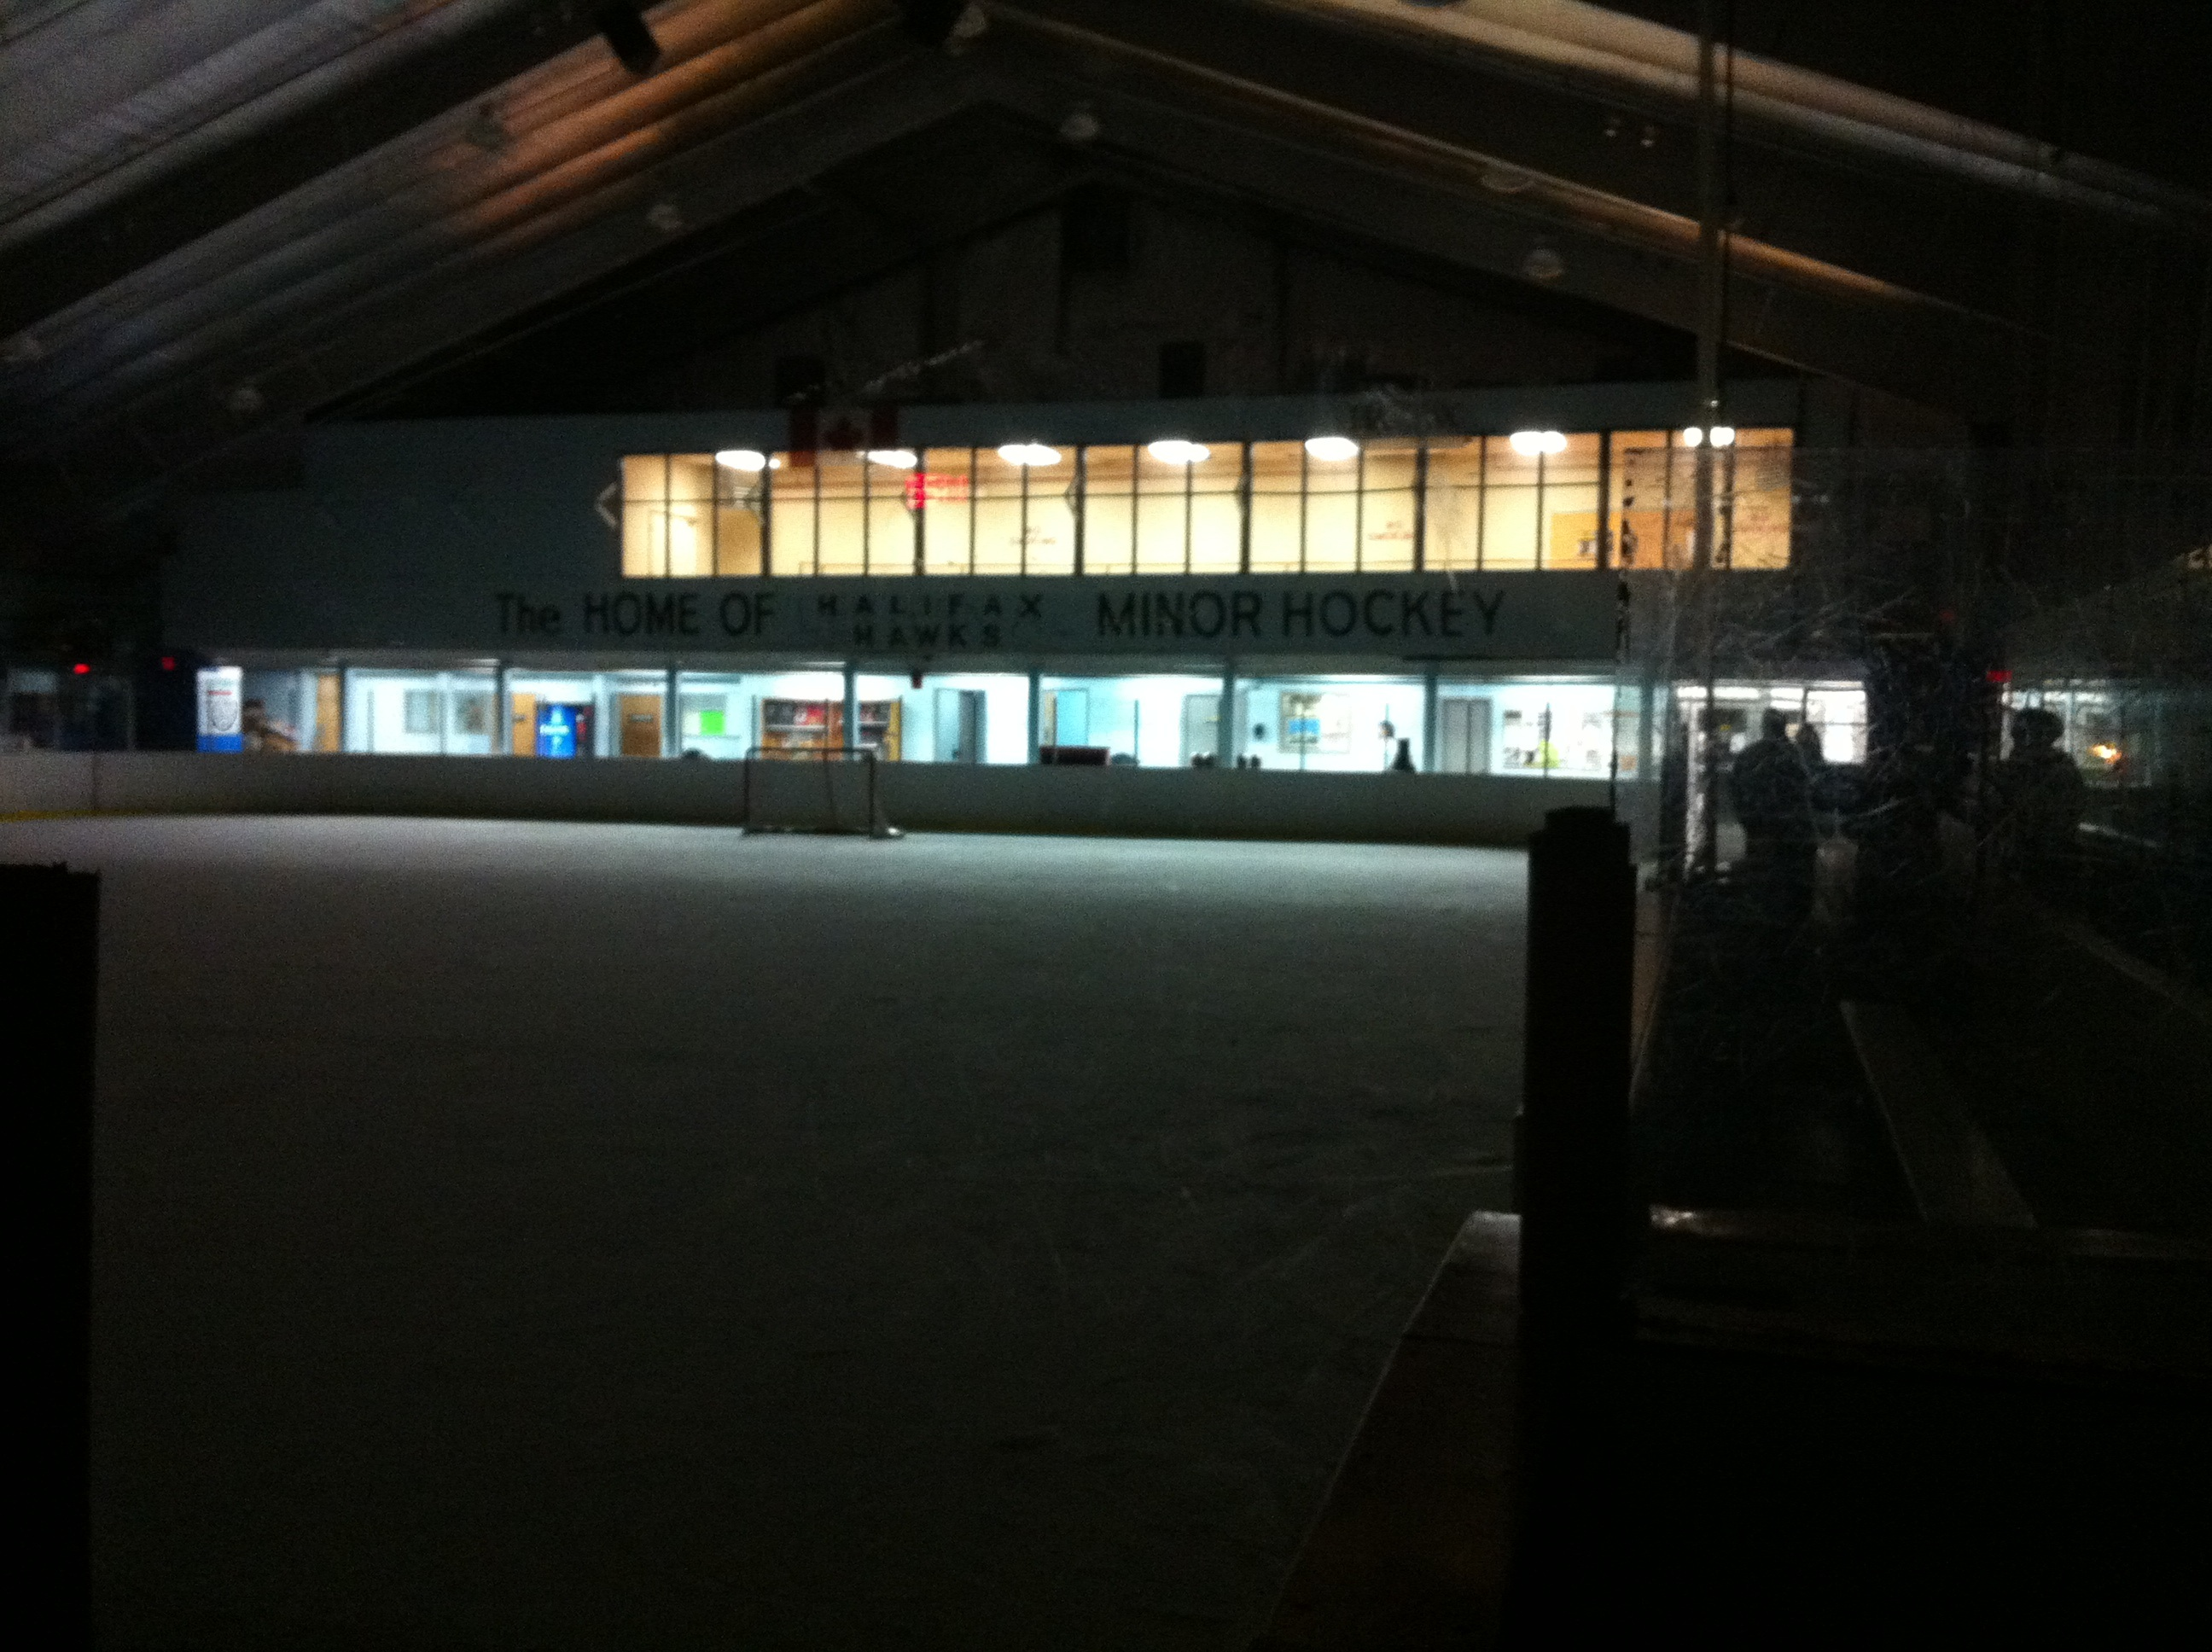
\includegraphics[width=0.30\linewidth]{images/rink.jpg} \\
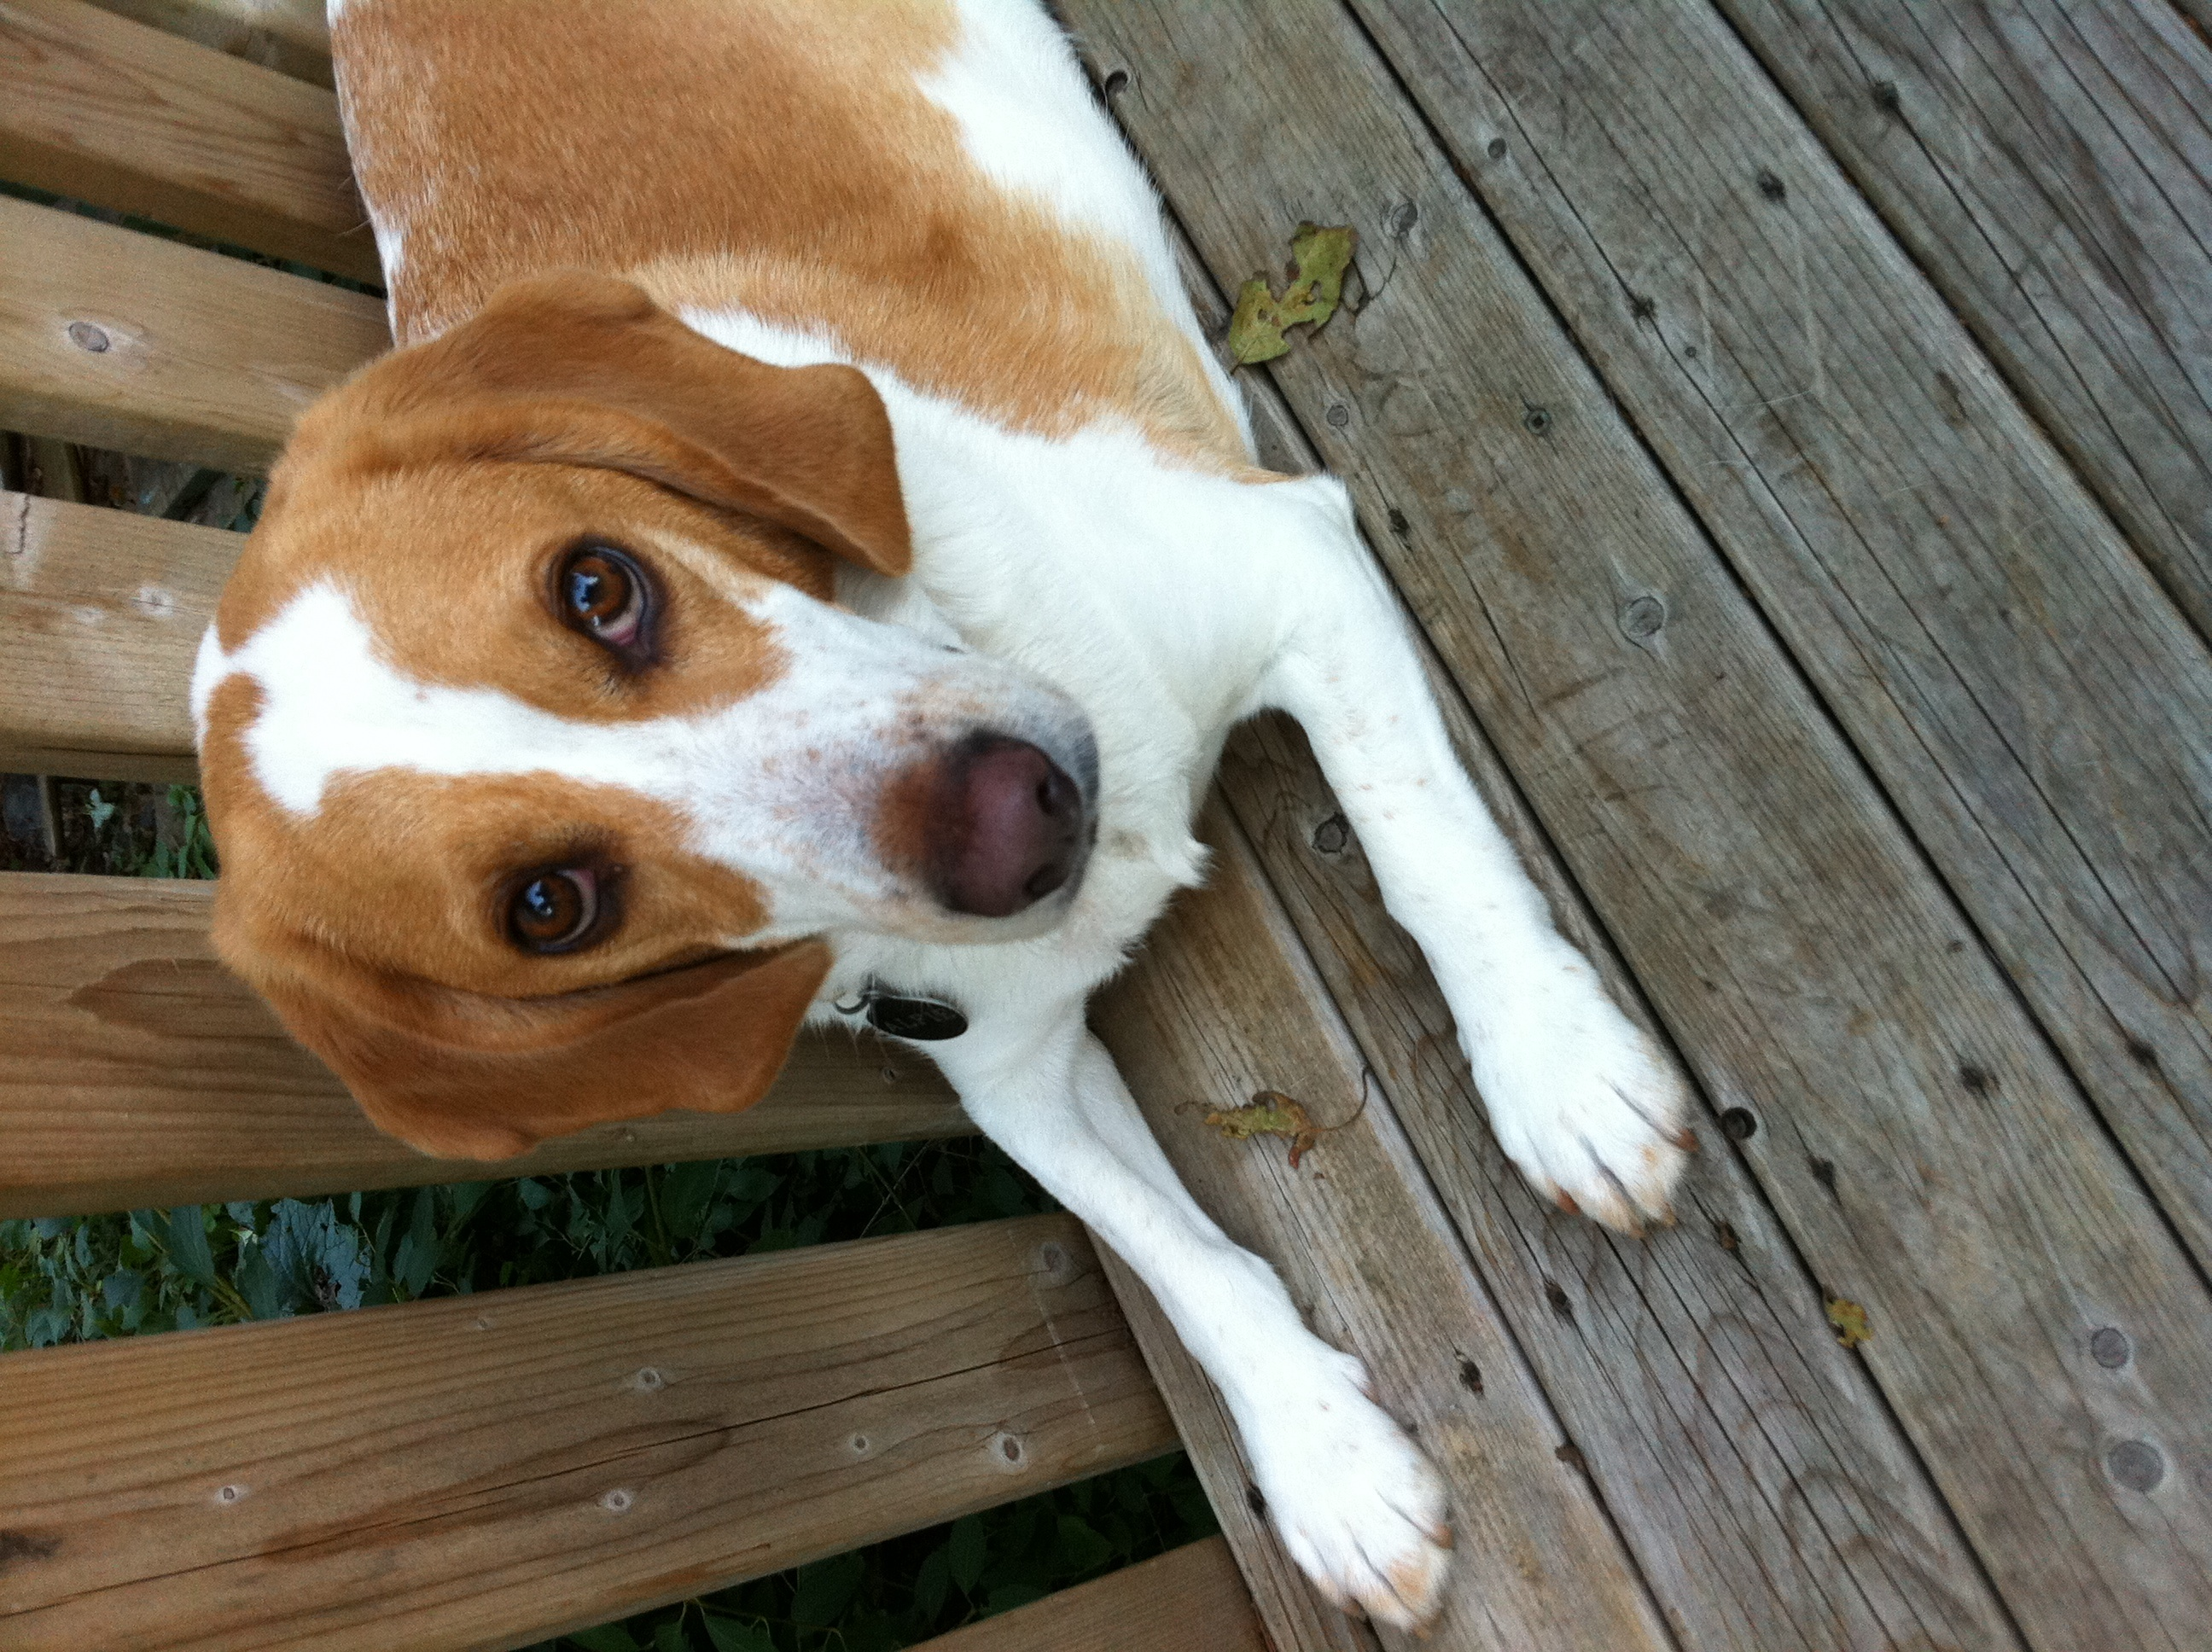
\includegraphics[angle=270, origin=c, width=0.30\linewidth]{images/alfie.jpg}&
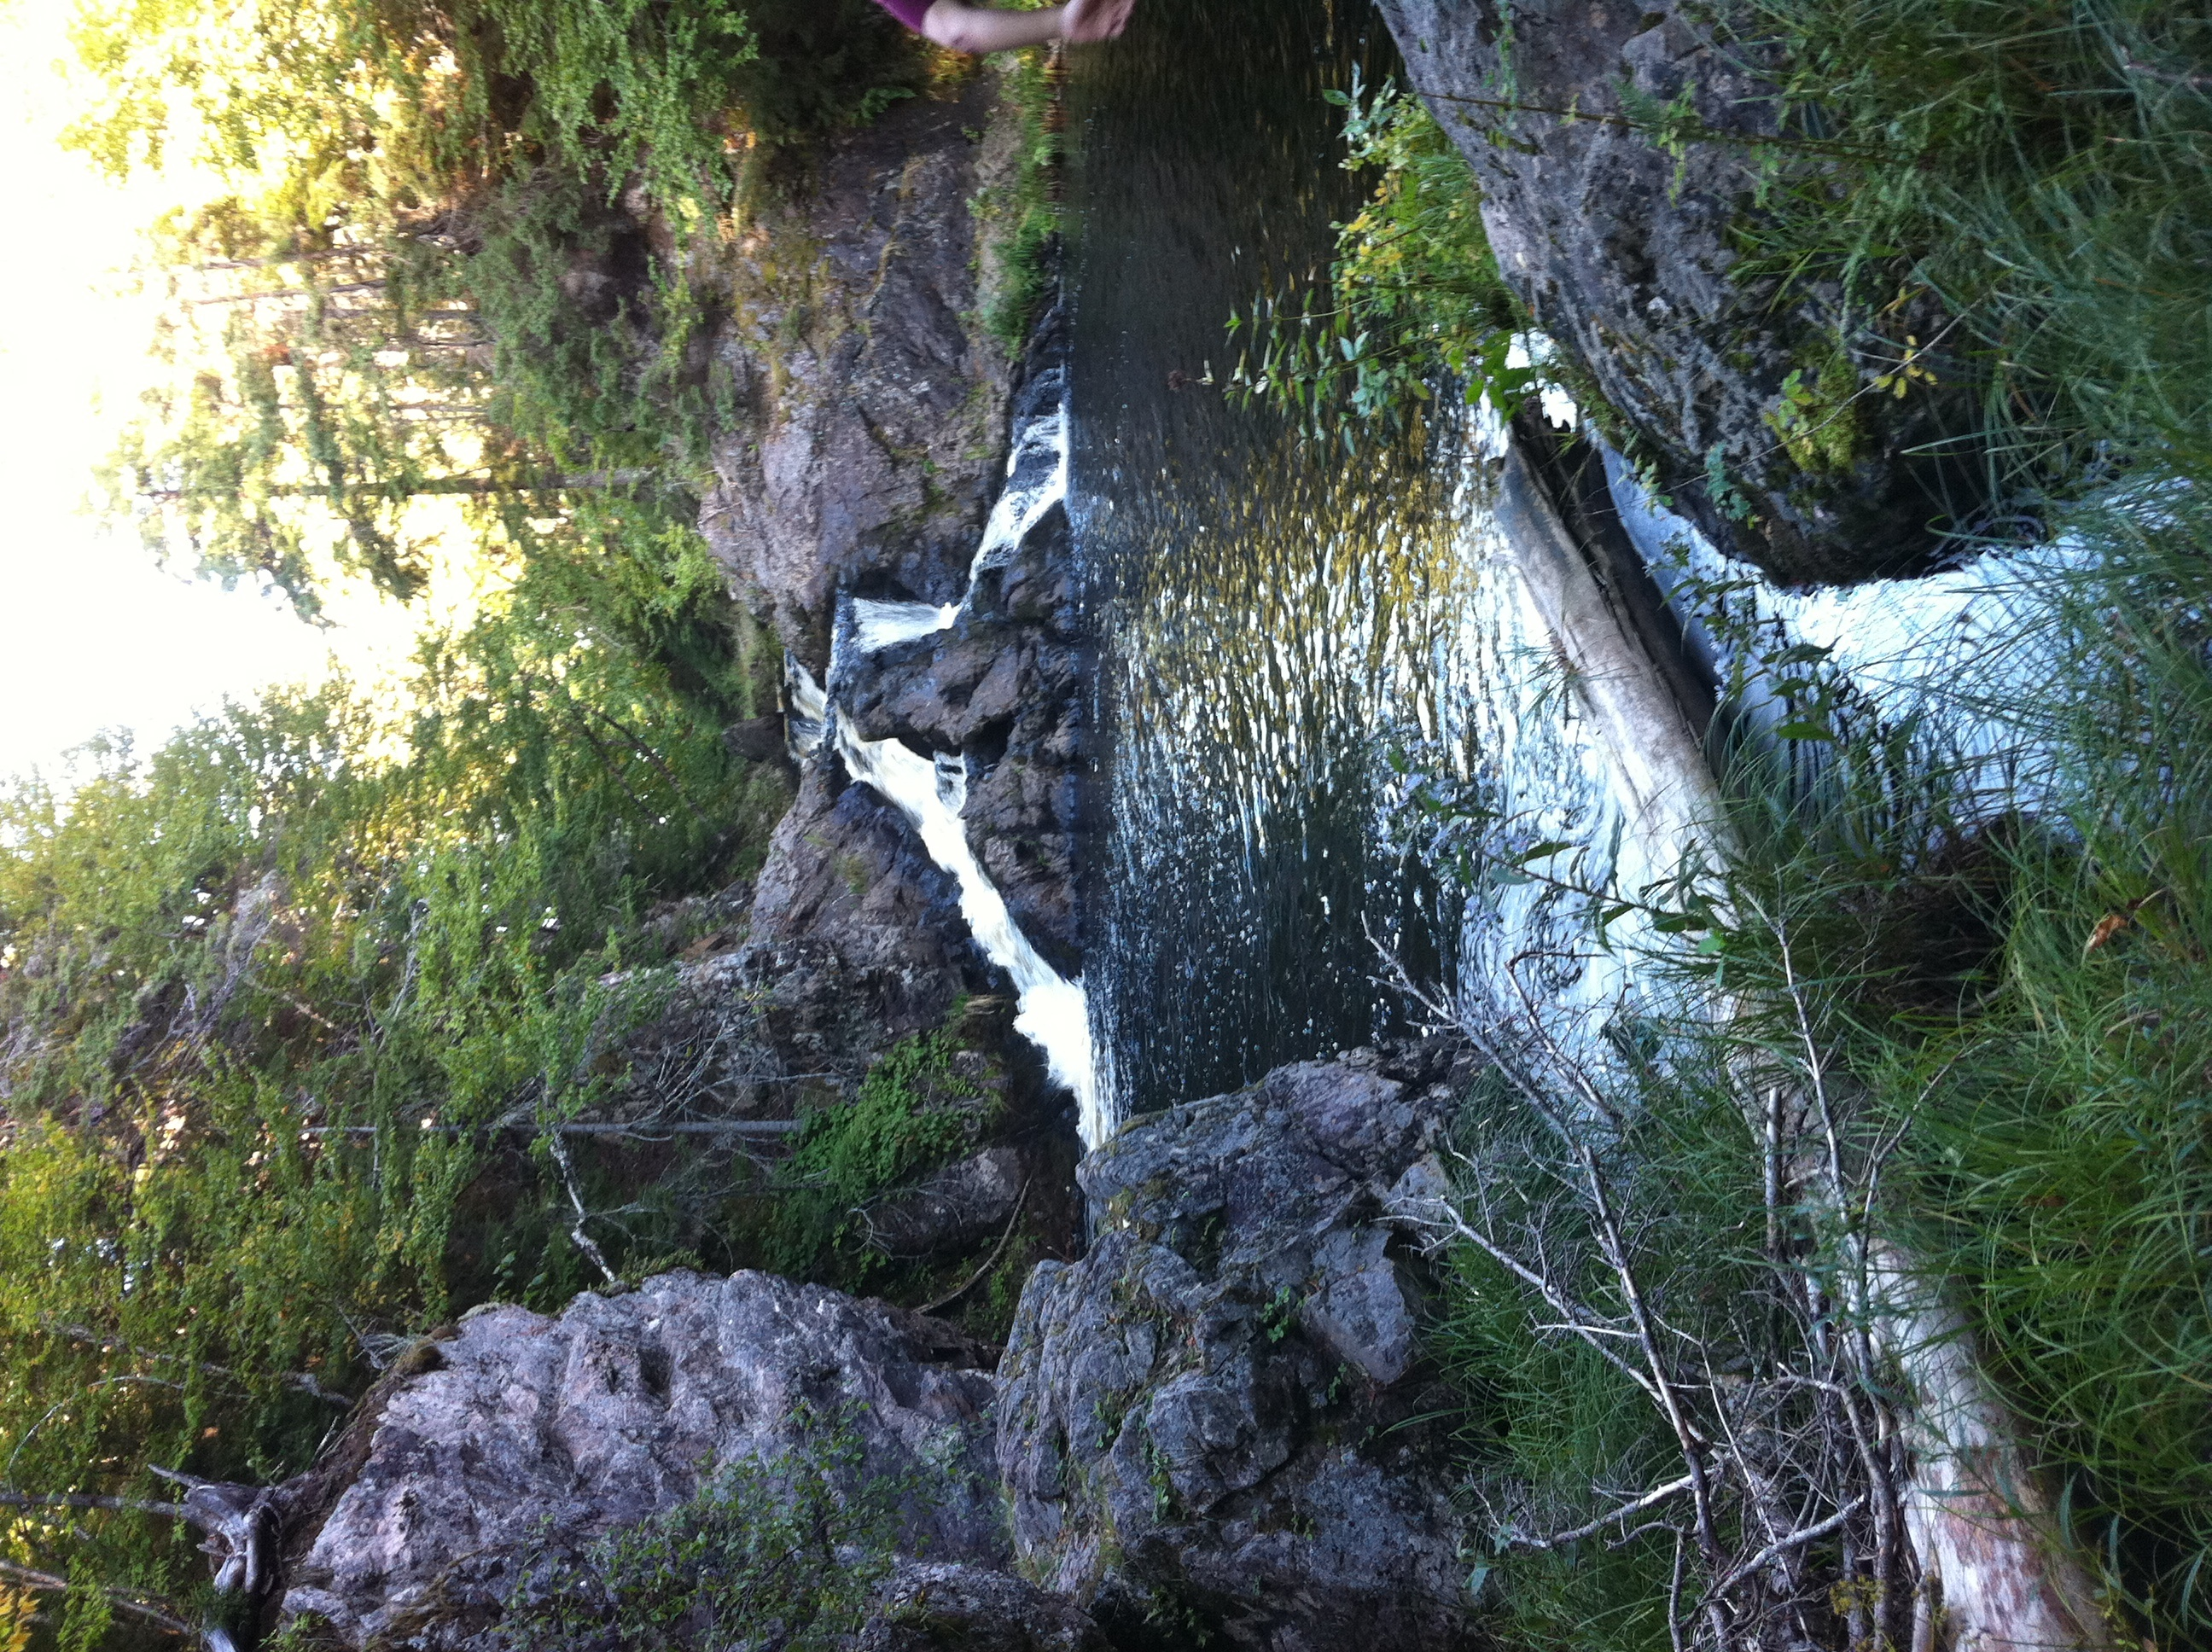
\includegraphics[angle=270, origin=c, width=0.30\linewidth]{images/camping.jpg}\\
\end{tabular}

\end{frame}

\begin{frame}
\frametitle{Where I'm from}
\framesubtitle{Atlantic Canada}
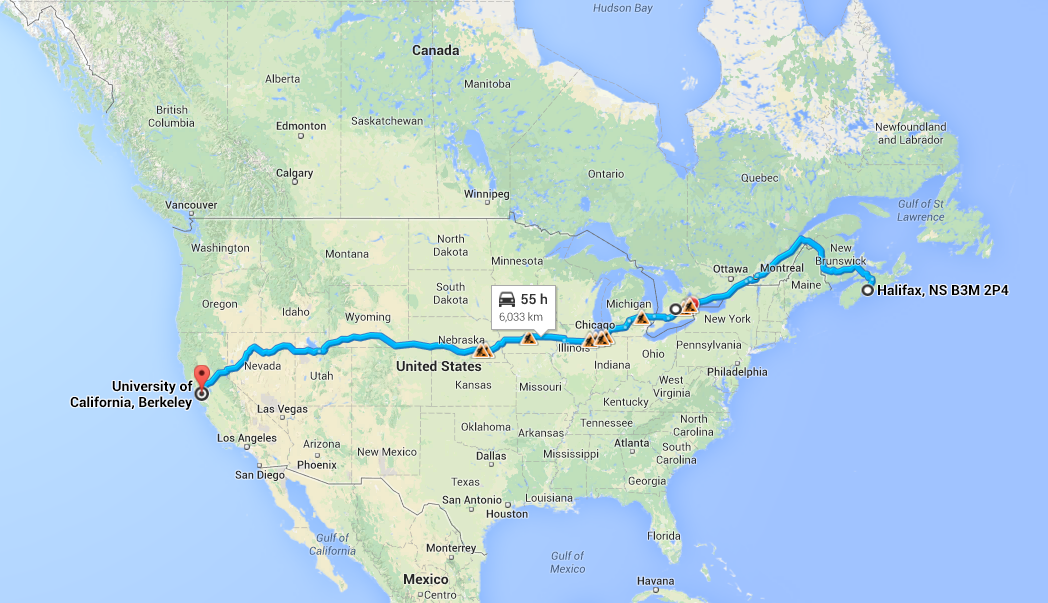
\includegraphics[width=1.0\linewidth]{images/map.png}
\end{frame}

\begin{frame}

\frametitle{What I'm Studying}

\begin{columns}[l]
\begin{column}{.7\textwidth}
\begin{description}
\item[Year] 2
\item[Program] Bachelor of Computer Science
\item[Faculty] Mathematics
\item[Institution] University of Waterloo
\item[Location] Waterloo, Ontario, Canada
\end{description}
\end{column}
\begin{column}{.3\textwidth}
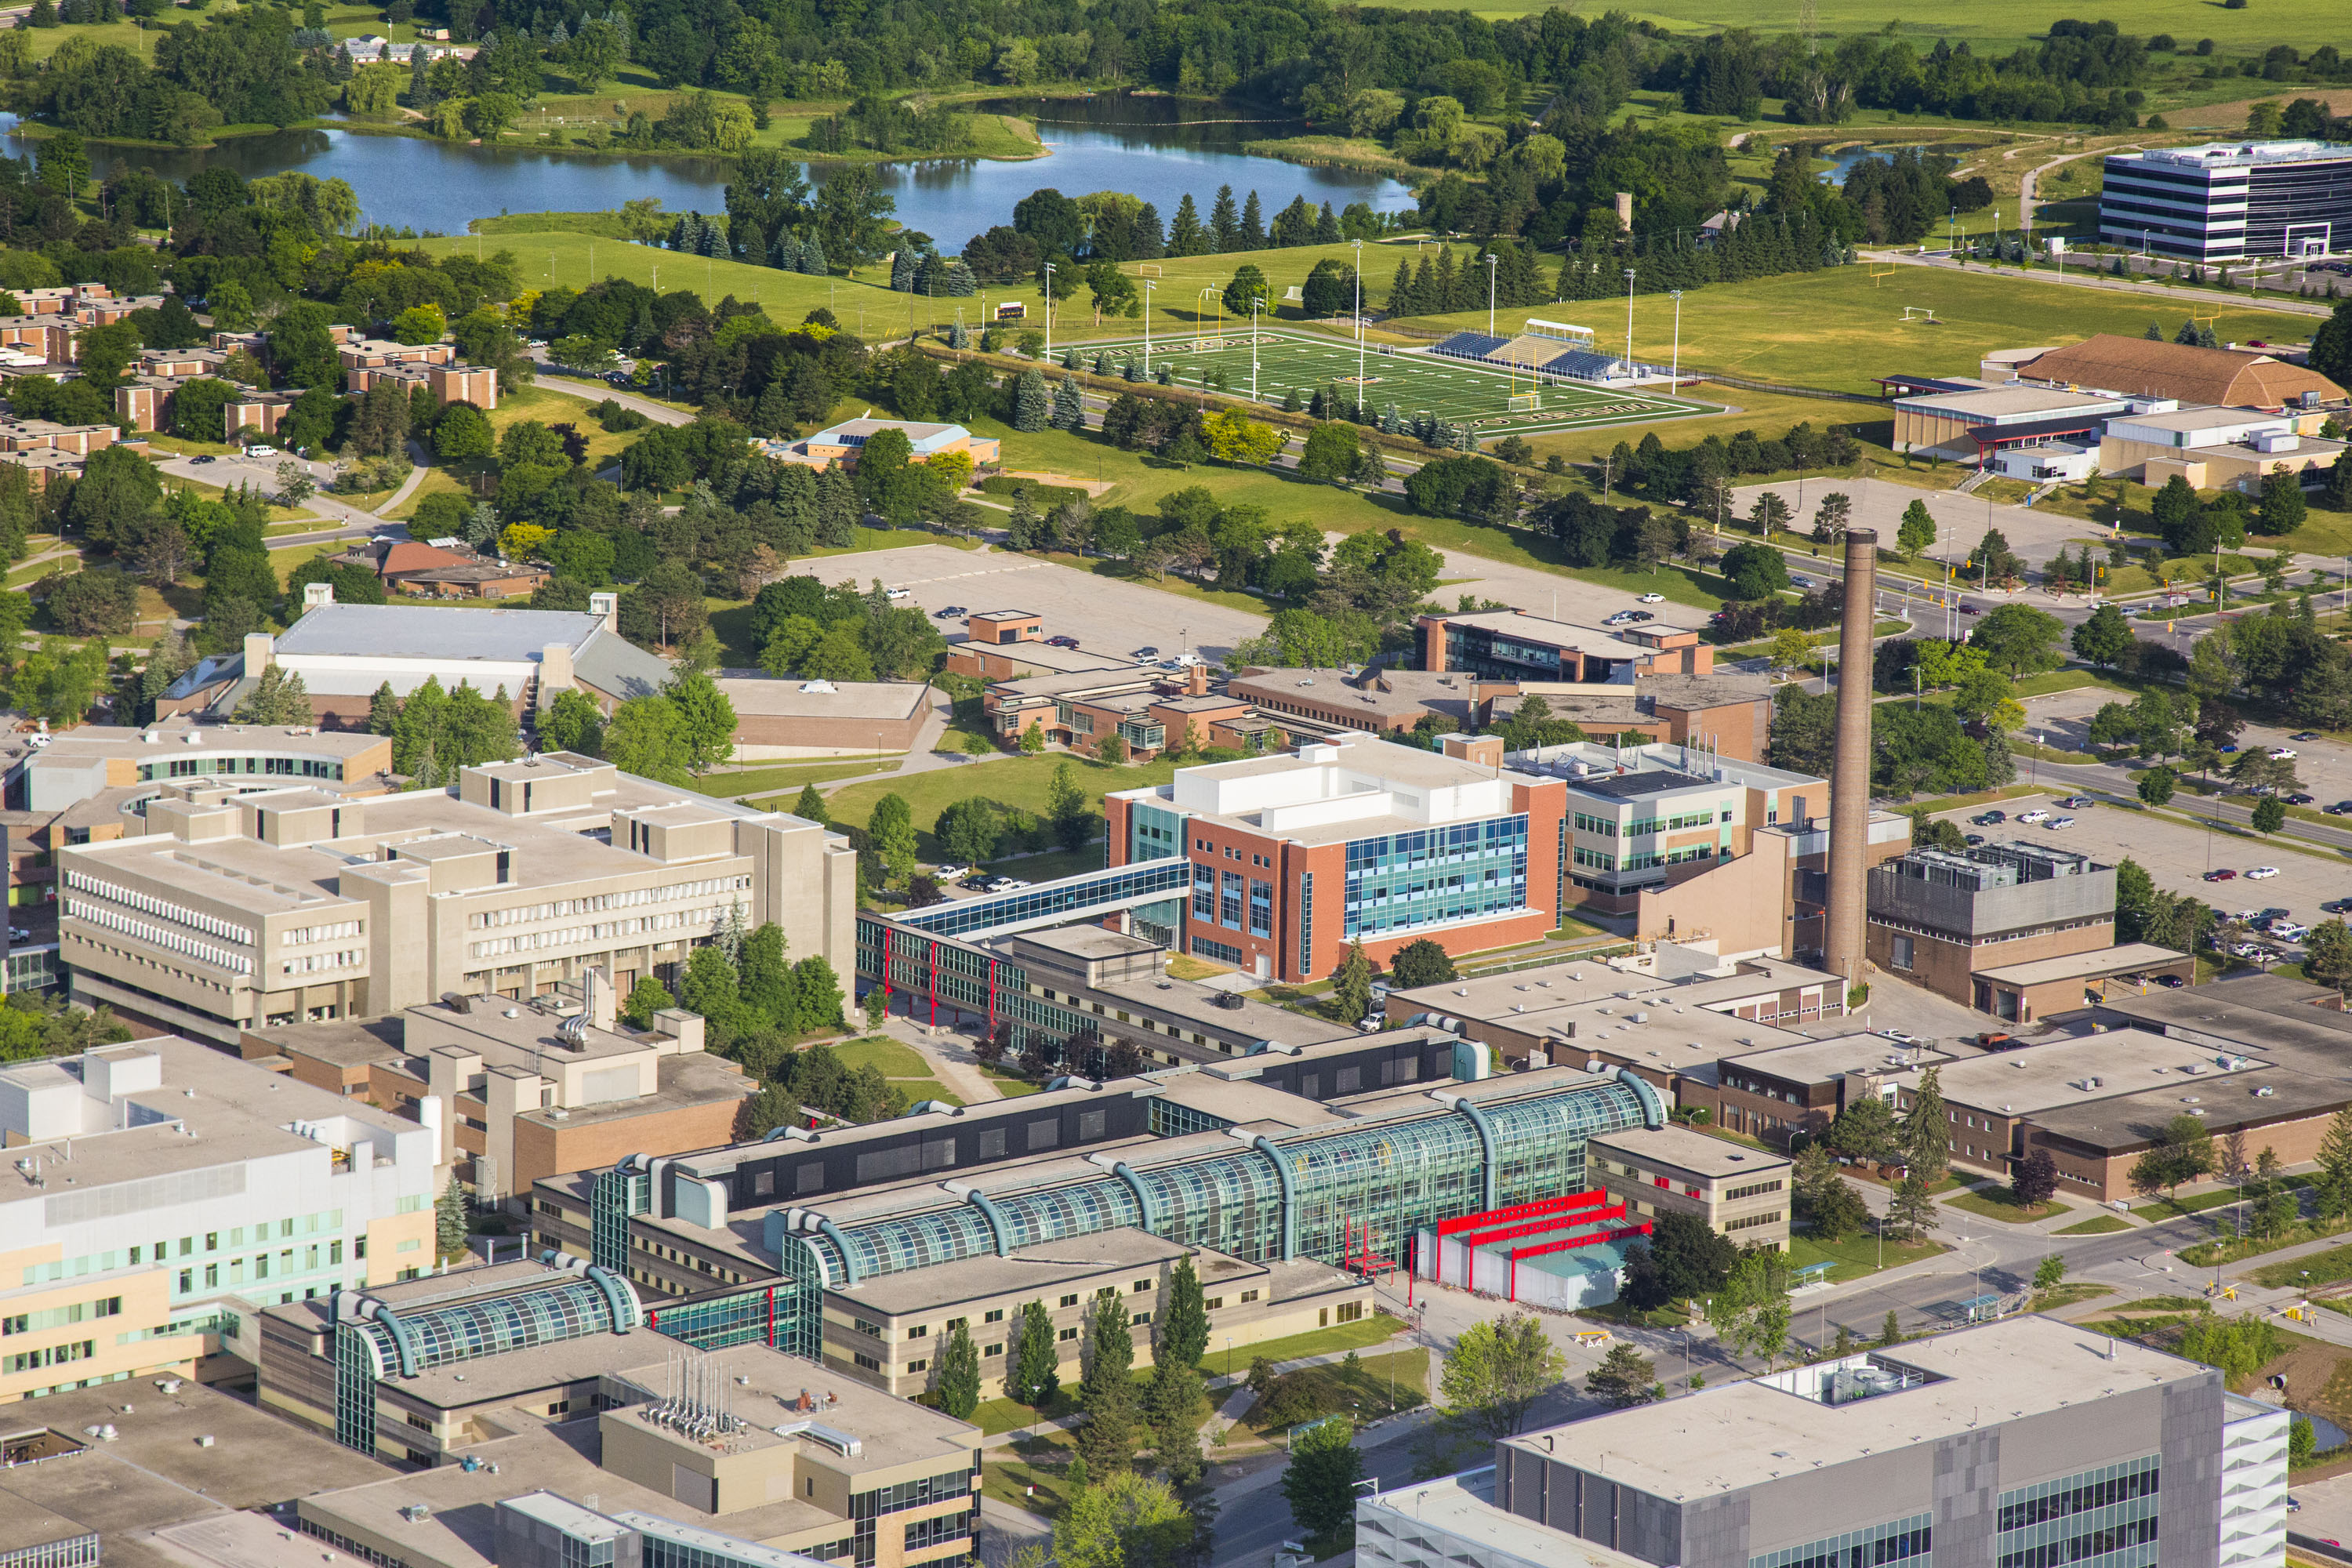
\includegraphics[width=1.0\linewidth]{images/campus.jpg}
\end{column}
\end{columns}

\end{frame}

\begin{frame}

\frametitle{How I Became a Researcher at CREA}
\framesubtitle{Prof. Garan Emailed the University of Waterloo Computer Science Club}

\centering

\begin{tabular}{c c}
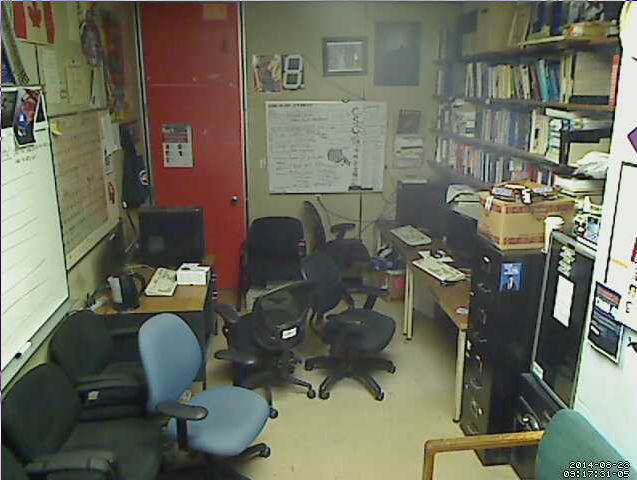
\includegraphics[width=0.40\linewidth]{images/malto_webcam.png} &
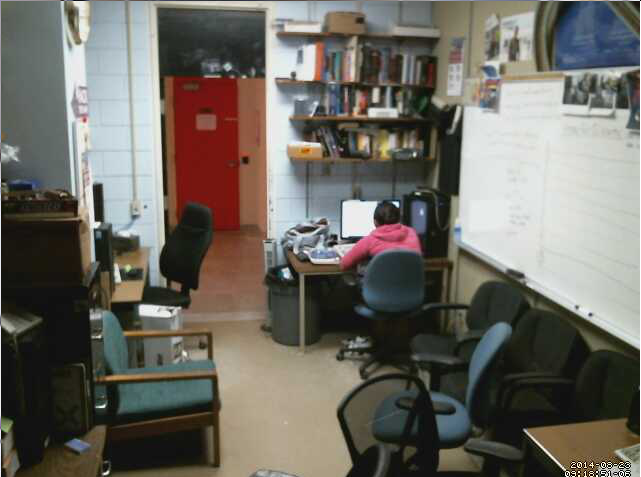
\includegraphics[width=0.40\linewidth]{images/bitshift_webcam.png}\\

\includegraphics[width=0.40\linewidth]{images/csc.png} &
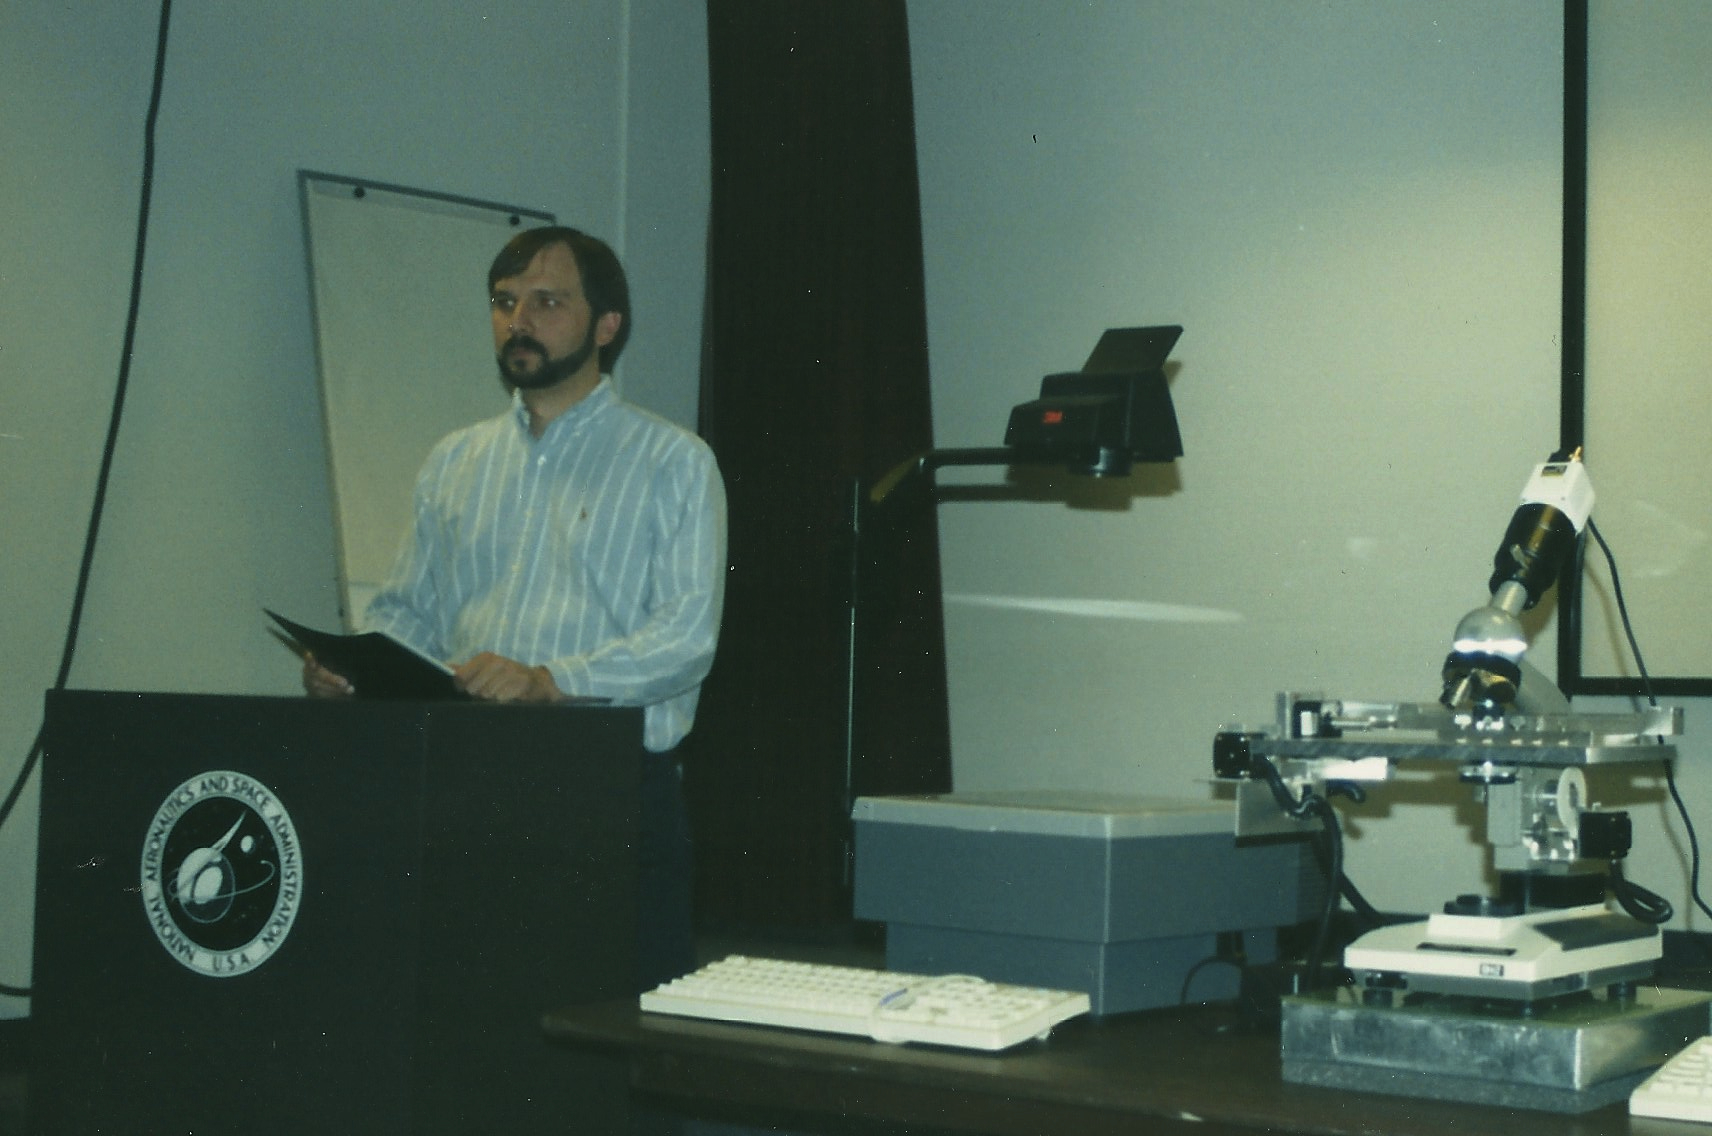
\includegraphics[width=0.40\linewidth]{images/steve_garan.jpg}\\
\end{tabular}

\end{frame}

\begin{frame}

\frametitle{Why was I Interested in Research at CREA?}

\centering
\begin{tabular}{ c | c }
Hobby & CREA Research \\
\hline
Reverse Engineering & Natural Language Processing\\
Game Development & Artificial Intelligence\\
Health & Bioinformatics\\
\end{tabular}

\end{frame}

\section{Understanding Aging}

\begin{frame}

\frametitle{What does CREA want to do?}
\framesubtitle{CREA Wants to Understand Aging and Increase Human Lifespan}

\centering

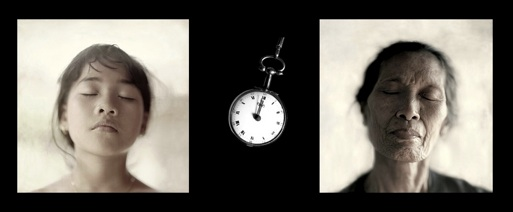
\includegraphics[width=0.75\linewidth]{images/aging.jpg}

% New discoveries are published quickly and in large volume.
% It is infeasible to construct the knowledge base by hand.
% Working on software to construct the knowledge base automatically.

\end{frame}

\begin{frame}

\frametitle{Why is it Difficult to Understand Aging?}

\centering
\only<1>{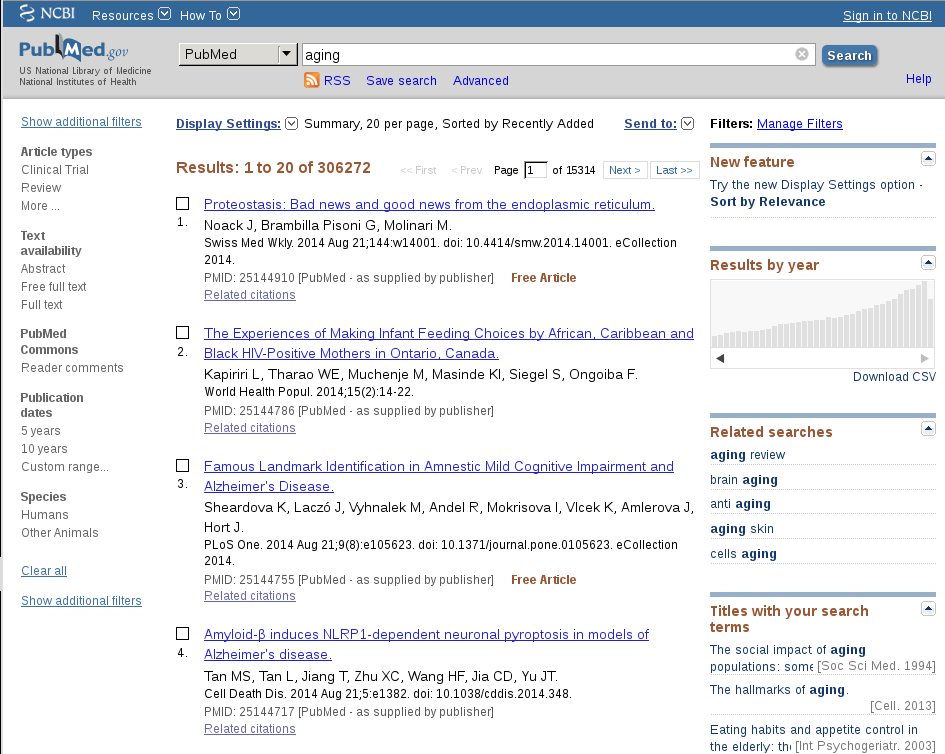
\includegraphics[width=.75\linewidth]{images/pubmed.png}}
\only<2>{
\includegraphics[width=.5\linewidth]{images/cascadeofbooks.jpg}}

\end{frame}

\begin{frame}

\frametitle{How can CREA Understand Aging?}
\framesubtitle{Build a Knowledge Base that Describes and Reasons about Aging}

\centering
\only<1>{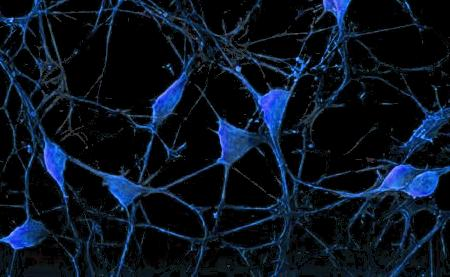
\includegraphics[width=1.0\linewidth]{images/knowledgebase.jpg}}
\only<2>{

\tikzstyle{decision} = [diamond, draw, fill=blue!60,
text width=4.5em, text badly centered, node distance=3cm, inner sep=0pt]
\tikzstyle{block} = [rectangle, draw, fill=blue!60,
text width=5em, text centered, rounded corners, minimum height=4em]
\tikzstyle{line} = [draw, -latex']
\tikzstyle{cloud} = [draw, ellipse,fill=red!60, node distance=3cm,
minimum height=2em]

\begin{tikzpicture}[scale=1, node distance = 2cm, auto]
\node [block] (acquire) {Acquire Biomedical Articles};
\node [block, below of=acquire] (extract) {Extract Knowledge};
\node [cloud, right of=acquire] (machine) {Machine};
\node [cloud, left of=acquire, node distance=4cm] (human) {Human};
\node [block, below of=human] (gui) {Graphical User Interface};
\node [decision, below of=extract] (belongs) {Is about Aging?};
\node [block, left of=belongs, node distance=4cm] (update) {Update Aging Theory};
\node [block, right of=belongs, node distance=4cm] (discard) {Discard};
\path [line] (acquire) -- (extract);
\path [line, dashed] (machine) -- (acquire);
\path [line, dashed] (extract) -| (machine);
\path [line] (extract) -- (belongs);
\path [line] (belongs) -- node{yes}(update);
\path [line] (belongs) -- node{no}(discard);
\path [line, dashed] (human) -- (acquire);
\path [line, dashed] (human) -- (gui);
\path [line] (gui) -- (update);
\end{tikzpicture}

}

% Routinely search for keywords related to aging, dowloading text articles from sources like PubMed.
% Build a spam filter to get rid of non-scientific sentences.
% Extract scientific facts from the sentences and save them in a structured format.
% Provide a graphical interface that allows users to search and explore the knowledge base.

\end{frame}

\section{Knowledge Extraction}

\begin{frame}

\frametitle{Knowledge Extraction}
\framesubtitle{Overview of Progress}

\centering

\begin{block}{Input}
... The \textcolor{orange}{pyridinoline} and \textcolor{orange}{desmosine}
were \textcolor{pink}{examined} as \textcolor{orange}{candidate sensitizer chromophores}
\textcolor{pink}{contained} in \textcolor{orange}{collagen} and \textcolor{orange}{elastin},
respectively. ...
\end{block}

\begin{block}{Output}
\centering
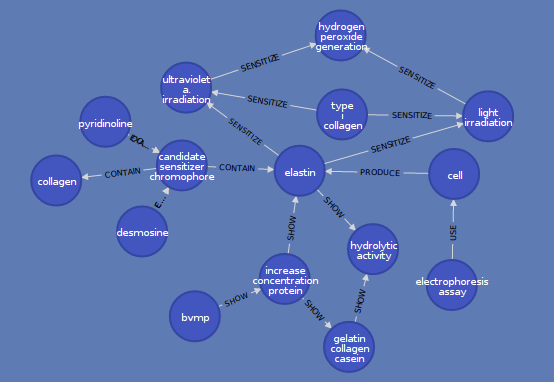
\includegraphics[width=0.5\linewidth]{images/elastinneighborhood.png}
\end{block}

\end{frame}

\begin{frame}

\frametitle{Knowledge Extraction}
\framesubtitle{Method}

\begin{description}[<+->]

\item[Tokenization] Input a text document and read it, one sentence at a time.
\item[Parsing] For each sentence, generate a constituent tree that describes its phrase structure.
\item[Compilation] Extract facts by pattern matching on each constituent tree.

\end{description}

\end{frame}

\begin{frame}

\frametitle{Constituent Tree Tags}
\framesubtitle{Word Level}

\centering

\begin{tabular}{c | c | c}
Tag & Meaning & Example \\
\hline
DT & Determiner & the \\
IN & Preposition & of\\
JJ & Adjective & blue\\
RB & Adverb & quickly\\
CC & Coordinating Conjunction & and \\
NN & Singular Noun & monkey\\
NNS & Plural Noun & monkeys\\
VB & Base Verb & fall\\
VBZ & Singular Present Verb & falls\\
VBD & Past Tense Verb & fell\\
VBN & Past Participle Verb & fallen\\
VBG & Gerund Verb & falling\\
... & ... & ...\\
\end{tabular}

\end{frame}

\begin{frame}

\frametitle{Constituent Tree Tags}
\framesubtitle{Phrase Level}

\centering

\begin{tabular}{c | c | c}
Tag & Meaning & Example \\
\hline
NP & Noun Phrase & the woman \\
VP & Verb Phrase & calls the man \\
PP & Prepositional Phrase & from the store \\
ADVP & Adverb Phrase & quickly and quietly \\
ADJP & Adjective Phrase & blue and red \\
CONJP & Conjunctive Phrase & as well as \\
... & ... & ...\\
\end{tabular}

\end{frame}


\begin{frame}

\frametitle{Constituent Tree Tags}
\framesubtitle{Clause Level}

\centering

\begin{tabular}{c | c | c}
Tag & Meaning & Example \\
\hline
S & Declarative Clause & the dog walks\\
SBAR & Conjunction + Clause & that the dog walks\\
... & ... & ...\\
\end{tabular}

\end{frame}

\begin{frame}

\frametitle{Knowledge Extraction}
\framesubtitle{Example}

\only<1>{
\begin{block}{Input Token}
The man walks the dog.
\end{block}
}

\only<2>{
\begin{block}{Parse Token}
\Tree [.ROOT [.S [.@S [.NP [.DT The ] [.NN man ] ] [.VP [.VBZ walks ] [.NP [.DT the ] [.NN dog ] ] ] ] [.. ] ] ]
\end{block}
}

\only<3>{
\begin{block}{Compile Token}
\Tree [.ROOT [.S [.@S [.NP [.DT The ] [.NN man ] ] [.$\langle$predicate:walk$\rangle$ [.NP [.DT the ] [.NN dog ] ] ] ] [.. ] ] ]
\end{block}
}

\only<4>{
\begin{block}{Compile Token}
\Tree [.ROOT [.$\langle$predicate:walk$\rangle$ [.NP [.DT The ] [.NN man ] ] [.NP [.DT the ] [.NN dog ] ] ] ]
\end{block}
}

\only<5>{
\begin{block}{Compile Token}
\Tree [.ROOT [.$\langle$predicate:walk$\rangle$ $\langle$argument:man$\rangle$ $\langle$argument:dog$\rangle$ ] ]
\end{block}
}

\only<6>{
\begin{block}{Output Fact}
\centering
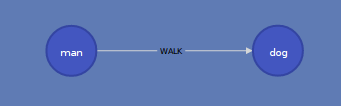
\includegraphics[width=.5\linewidth]{images/manwalkdog.png}
\end{block}
}

\end{frame}

\begin{frame}

\frametitle{Software Demonstration}
\framesubtitle{A preview of CREA's knowledge base, compiled from PubMed abstracts.}

\href{http://markfarrell.ca/creal}{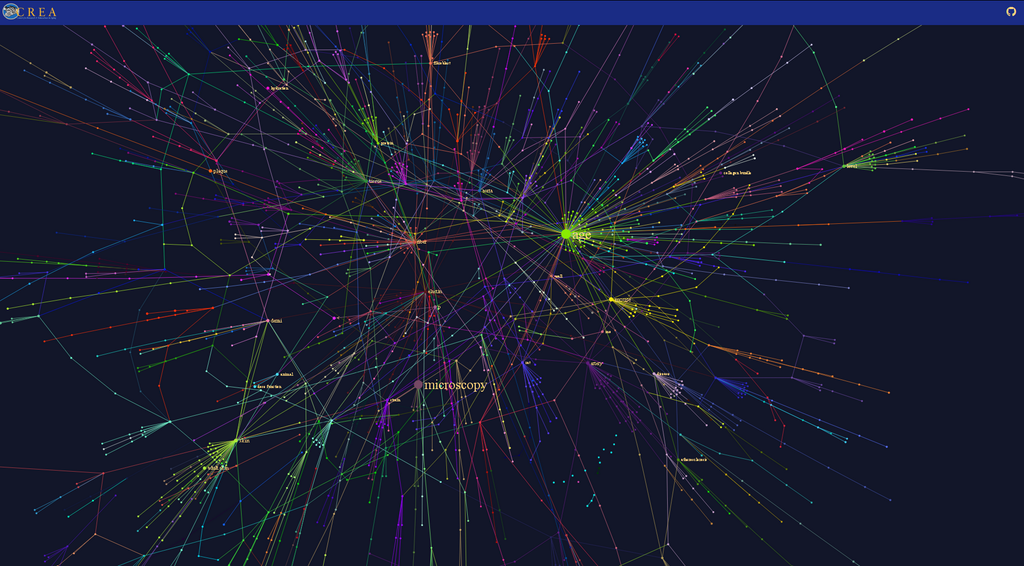
\includegraphics[width=1.0\linewidth]{images/results.png}}

\end{frame}

\begin{frame}

\frametitle{High Performance}
\framesubtitle{Knowledge can be extracted from many sentences at the same time.}

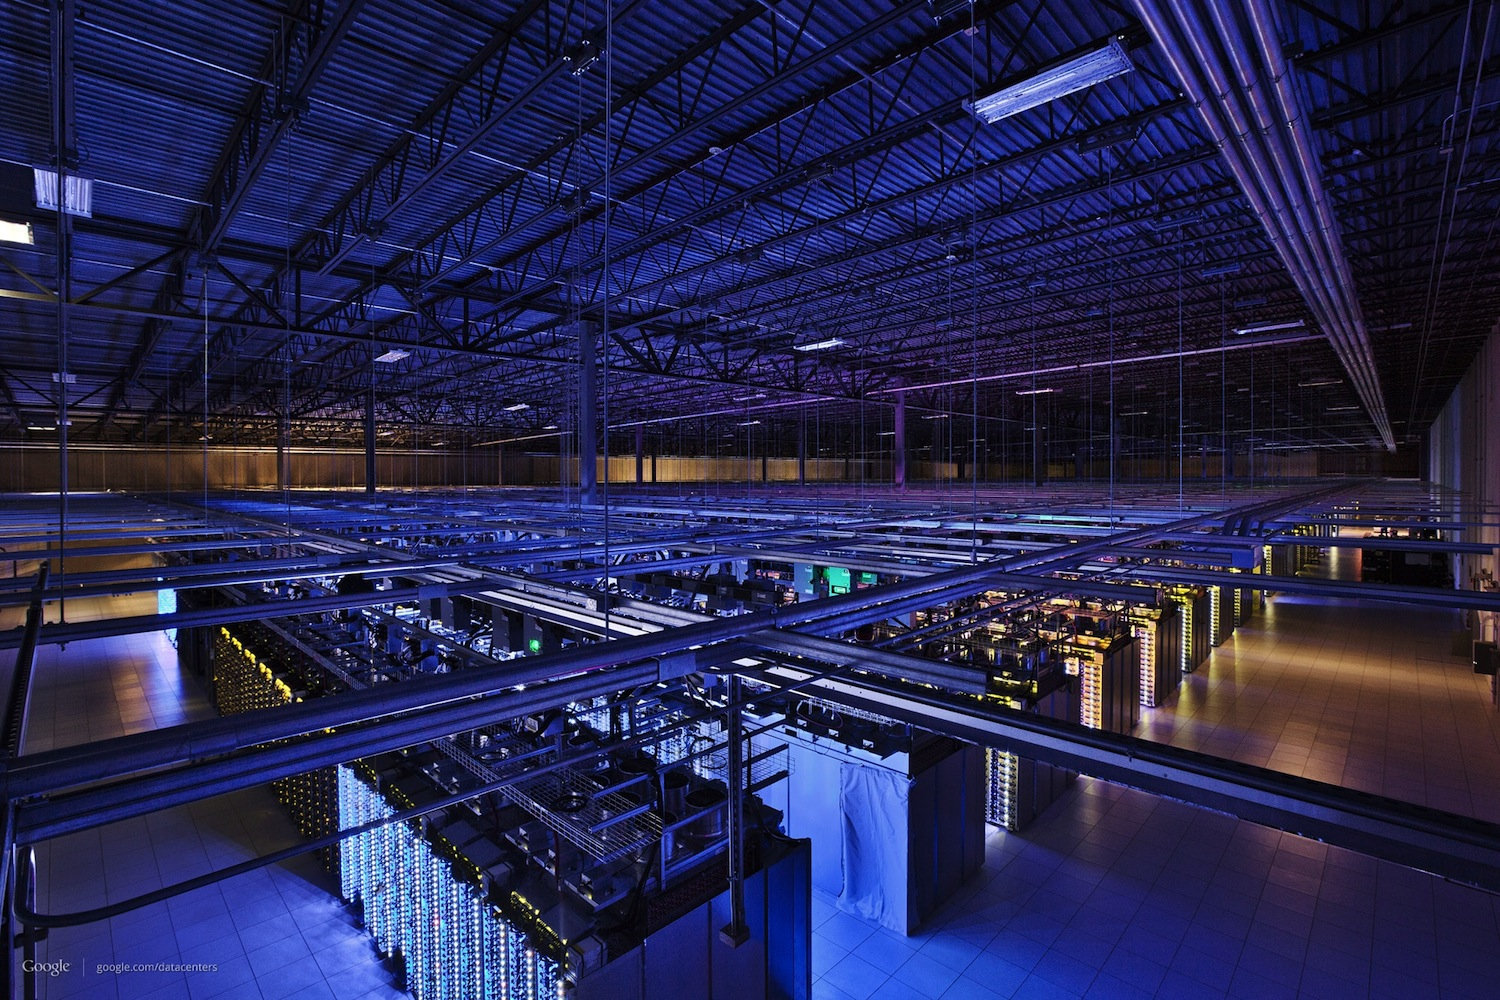
\includegraphics[width=1.0\linewidth]{images/parallel.jpg}

\end{frame}

\section{What Next?}

\begin{frame}

\frametitle{What Next?}

\centering

\begin{tabular}{c | c}
Task &  Assignees\\
\hline
\textcolor{green}{Research Direction} & \textcolor{green}{Steve Garan} \\
\textcolor{yellow}{Knowledge Extraction} & \textcolor{yellow}{Mark Farrell} \\
\textcolor{yellow}{Text Article Retrieval} & \textcolor{yellow}{Grace Park, Jeremy Wan} \\
\textcolor{yellow}{Knowledge Visualization} & \textcolor{yellow}{Mark Farrell} \\
\textcolor{orange}{Graphical User Interface} & \textcolor{orange}{Mark Farrell} \\
\textcolor{red}{Biomedical Spam Filtering} & \textcolor{red}{---} \\
\textcolor{red}{Automated Reasoning} & \textcolor{red}{---} \\
\end{tabular}


% Filter spam sentences from documents.
% The accuracy of the parser could be optimized:
% Should be trained to identify more nouns from the biomedical domain.
% Define more patterns for extracting facts: The software succeeds around 50\% of the time.


% Support negated clauses and conditional logic.
% Facts can contradict each other:
% Store the probability that is true as the weight of its edge on the
% knowledge base's graph.
% Scale and launch the software service.

% Demonstrated a method for automatically constructing CREA's
% knowledge base on aging.
% Showed how to extract facts from English text in the knowledge
% base's structured format.
% Discussed the need to improve software accuracy by lensing in on
% the biomedical domain.
% Suggested how the software implementation can be scaled for
% production usage.

\end{frame}

\begin{frame}

\frametitle{Get Involved}
\framesubtitle{Contact Me for More Information}

\begin{description}
\item[Email] m4farrel@csclub.uwaterloo.ca
\item[Website] markfarrell.ca
\end{description}

\end{frame}

\end{document}
